\documentclass[11pt]{article}
\usepackage[T1]{fontenc}
\usepackage{lmodern}
\usepackage[margin=2.3cm]{geometry}
\usepackage{booktabs,tabularx,array}
\newcolumntype{Y}{>{\raggedright\arraybackslash}X}
\usepackage{xcolor}
\usepackage{amsmath,amssymb}
\usepackage{graphicx}
\usepackage{enumitem}
\usepackage[colorlinks=true,linkcolor=blue!50!black,urlcolor=blue!50!black,citecolor=blue!50!black]{hyperref}
\setlist{nosep,leftmargin=*}
\emergencystretch=2em
\newcommand{\code}[1]{\texttt{#1}}
\newcommand{\E}[1]{E#1}

\title{Writing Tiled Kernels with an 8B Model under an 8k-Token Budget:\\[2pt]
\large Put the Rules in the Verifier, Translate Verdicts into One Instruction}
\author{Team seats 130, 132, 133, 134}
\date{2026-10-10}

\begin{document}
\maketitle

\begin{abstract}
\noindent
A small model (Qwen3-8B, 8192 tokens per call including the answer) must write tiled,
explicit-memory kernels for a ten-level operation ladder under accelerator rules (tiles of at most
$128\times512$, explicit loops, no fancy indexing or broadcasting, no calling the op, correct partial
tiles). Putting the rules in the prompt makes the model audit itself into silence; leaving them out
yields confident illegal code. We move every rule into a verifier and turn each verdict into one
instruction. The verifier checks rules in two layers (AST and a runtime NumPy proxy), accepts a
result if it lies within a proven float32 forward-error bound $\gamma_k\cdot s$, and explains failures by
cross-case patterns and numerically verified hypotheses rather than diffs. The agent sends a
one-sentence first prompt and thereafter the previous code plus one directive. With everything
else equal, translated directives verify 15 of 20 runs on levels 1--4 against 4 of 20 when the
verdict is sent back verbatim. Levels 4 and above remain a wall (v2: 1/5 on L4, 0/5 on L5--L7).
A second stage makes verified kernels cheaper without making them wrong: 5 of 11 rewrites accepted,
up to $79\times$ fewer instructions. The largest prompt was 706 tokens (13\% of the input budget), so
in Stage~A the budget never binds. Under the organizers' own checker, every verified kernel on L1--L3
passes 32/32 and the verified L6 kernel passes; L4/L8 fail on a signature mismatch and L7/L10 on a
per-element tolerance stricter than our bound. A pre-registered test adopted v3 (3 of 9 runs verified on
L4--L6 against v2's 1 of 25); the final agent, v4, adds the organizers' checker as an acceptance gate,
and its runs are pending.
\end{abstract}

\tableofcontents

%==============================================================================
\section{Introduction}

The visible task is to write kernels. The real task is \emph{context selection}: every model call
sees at most 8192 tokens, input and output together, while documentation, specification, reference,
the current kernel and the last failure do not fit at once. Each round, someone has to decide what
goes on that one page.

The obvious answer, ``put the rules on the page'', fails in a specific way. A prompt full of
prohibitions makes an 8B model check itself against every rule in a loop and return nothing; the
upstream agent measured that a 1866-character prompt yields no code where a 581-character prompt
does. The opposite, a one-sentence prompt, yields code at once, but code that calls \code{np.sum} and
scores zero. Neither is a page worth writing.

\paragraph{Thesis.} Rules belong in the verifier, not in the prompt. The model writes freely; the
verifier finds what is wrong with a proof-backed notion of ``wrong''; the agent translates that verdict
into one concrete change. The page then holds only the task, the current code and one instruction.

\paragraph{Contributions.}
\begin{itemize}
  \item A verifier that checks rules statically and at runtime, reports every violation by line in one
        execution, and accepts a numerical result iff it lies within a proven float32 error bound
        (\S\ref{sec:verifier}).
  \item Failure \emph{diagnosis}: cross-case patterns, common facts and level-specific hypotheses that
        are verified against the reference before they are stated (\S\ref{sec:diag}).
  \item An agent that turns each diagnosis into one directive and gates replies, with exact token
        accounting and a holdout-based confidence (\S\ref{sec:agent}).
  \item A controlled ablation: 15/20 vs 4/20 on L1--4 against the verbatim verdict, plus L5--L10 for
        both arms, a pre-registered v3 test (adopted: 3/9 vs 1/25), and an efficiency stage (\S\ref{sec:exp}).
  \item An honest account of where it fails: the L4 wall, oscillation, determinism, the unbinding
        budget in Stage~A, and disagreements with the organizers' checker (\S\ref{sec:analysis},
        \S\ref{sec:kb}).
\end{itemize}

%==============================================================================
\section{Setting}
\label{sec:setting}

\paragraph{Stage A rules.} A kernel is a NumPy function that imitates an accelerator:
\begin{itemize}
  \item every array it produces (operation result, slice, write region) is at most $128\times512$, a
        1-D array at most 512 long;
  \item it loops over tiles explicitly; whole-array operations are illegal by the rule above;
  \item no fancy or mask indexing, no broadcasting tricks (elementwise operands have identical shapes;
        scalars allowed; no \code{None}/\code{np.newaxis}, \code{keepdims}, reshape family);
  \item no calling the op: NumPy reductions, linalg, layout and index helpers are banned at every
        level, and so are builtin \code{sum/max/min} over iterables;
  \item the last tile is partial whenever a dimension does not divide; it must be handled.
\end{itemize}
Only \code{numpy} and \code{math} may be imported. Stage~B is the same problem in NKI on Trainium.

\paragraph{The ladder.} Ten levels: L1 \code{relu(a x + b)}, L2 row sum, L3 row max, L4 RMSNorm,
L5 softmax, L6 transpose, L7 matmul, L8 layernorm, L9 band attention, L10 conv1d.

\paragraph{Model and server.} Qwen3-8B on vLLM on a Trainium seat pod, thinking off,
\code{temperature=0.6}. Facts that shaped the design:
\begin{itemize}
  \item \code{max-model-len 8192} is input $+$ output; with a 2500-token answer reserve the prompt must
        stay under about 5.7k tokens. Near the limit the answer is silently truncated
        (\code{finish\_reason="length"}), so every reply is checked.
  \item Throughput is about 25 tokens/s per server, shared by all requests.
  \item The server is near-deterministic at \code{temperature=0.6}: two runs produced byte-identical
        code until the first divergence (\E{10}), and six requests of one prompt, four concurrent and two
        sequential, returned six byte-identical replies (\E{27}). A retry must change the prompt.
  \item A per-request \code{seed} kills the Neuron vLLM engine; every later request returns 500 (\E{5}).
        The client never sends it.
\end{itemize}

%==============================================================================
\section{The verifier}
\label{sec:verifier}

Built before the agent and validated on hand-written correct kernels (all pass, worst error
$8.4\times10^{-8}s$, \E{1}) and deliberately broken ones (all caught, each with the expected violation kind
and key phrase, \E{3}). Entry point: \code{uv run python -m kagent.harness LEVEL FILE}.

\subsection{Rules in two layers}
The \textbf{static layer} scans the AST, so it catches violations on code paths the test cases never
reach. The \textbf{runtime layer} executes the kernel with \code{numpy} replaced by a proxy whose arrays
are an \code{ndarray} subclass that \emph{records} each violation with its line instead of raising. One
execution therefore yields every broken rule and the numerical result. Violations on one line are
deduplicated (\code{np.sum} also trips \code{np.add.reduce}; only the specific one is shown).

A red-team kernel (PR~\#2) hid \code{xp = np; xp.max} on a branch the tests never take and passed the
static check with zero violations. Aliases are now propagated to a fixed point, with a regression test;
the runtime layer would have caught it had the branch executed.

\subsection{Tolerance as a proven bound}
\label{sec:tol}
A case passes iff for every output element
\[
  |y_{\text{got}} - y_{\text{ref}}| \;\le\; \gamma_k\, s,
  \qquad \gamma_k = \frac{k\,u}{1-k\,u},\quad u = 2^{-24},
\]
where $y_{\text{ref}}$ is computed in float64 on the exact float32 inputs, $s$ is the magnitude that
appears in the backward error analysis, and $k$ counts the roundings on the path to one output
(Higham, \emph{Accuracy and Stability of Numerical Algorithms}, ch.~3--4). Table~\ref{tab:bounds}
lists the bounds.

\begin{table}[h]
\centering\small
\begin{tabularx}{\linewidth}{@{}l>{\raggedright\arraybackslash}p{3.0cm}>{\raggedright\arraybackslash}p{4.6cm}Y@{}}
\toprule
Level & $k$ & $s$ & Diagnosis on failure \\
\midrule
1 relu & 3 & $|a||x|+|b|$ & -- \\
2 row sum & $N$ & $\sum_j|x_{ij}|$ & per-tile overwrite \\
3 row max & 0 (bit-exact) & $\max_j|x_{ij}|$ & per-tile overwrite; wrong identity \\
4 RMSNorm & $N+4$ & $|y|$ & per-tile mean square \\
5 softmax & $N+4$ & $y(1+|x-\max|)$, $+2^{-126}$ & per-tile softmax \\
6 transpose & 0 (exact) & -- & decode each wrong value to its source index \\
7 matmul & $K+1$ & $|A||B|$ & missing partial $K$ tile \\
8 layernorm & $N+6$ & $|g|(|\hat y|+\overline{|x|}/\sigma)+|b|$ & cancellation (mean$/\sigma\ge30$); per-tile statistic \\
9 band attention & $d+\min(2w{+}1,S)+8$ & $(p|v|)(1+\max|q||k|/\sqrt d)$, $+2^{-126}$ & band edge ($w\pm1$); one-sided window \\
10 conv1d & $C_{in}K+1$ & $|w|\star|x|$ & dilation ignored \\
\bottomrule
\end{tabularx}
\caption{Proven float32 bounds $\gamma_k s$ and the hypotheses each level tests on failure.}
\label{tab:bounds}
\end{table}

\paragraph{Why a bound and not a constant.} Our first tolerance was a chosen constant, $10^{-5}s$. A
logically correct row sum that accumulates in float32 failed it on \code{constant-rows 131x1031} with
error $1.5\times10^{-5}s$, and we ruled ``accumulate in float64'' (\E{2}). Under the proven bound,
$\gamma_{1031}s = 6.1\times10^{-5}s$, the same kernel is correct and uses 24\% of its bound (\E{7}): the
constant was rejecting a correct float32 algorithm. With the bound, the tolerance encodes what float32
can guarantee, not a preference. Bugs still fail by a wide margin (errors $\ge10^{-3}s$, against
$\gamma_{2053}=1.2\times10^{-4}$ at the longest row). Each pass reports its \emph{bound use}
$\max|y_{\text{got}}-y_{\text{ref}}|/(\gamma_k s)$: L1 47\%, L2 1\% (float64 accumulator) or 24\%
(float32), L3 0\%; hand kernels on L4--L7 use at most 44\%, and a legal float32 two-pass layernorm 25\%
while $E[x^2]-E[x]^2$ fails on exactly the large-mean and constant rows. Errors above the bound but
below $10^{-3}s$ are labelled rounding-sized, so the agent does not hunt for a logic bug.

\subsection{Diagnosis instead of verdicts}
\label{sec:diag}
A failure report is ordered by how much it narrows the search:
\begin{enumerate}
  \item \textbf{Cross-case tag pattern.} Each case has shape tags (\code{partial-col-tile},
        \code{dim-1}, \code{prime-dim}, \dots) and a value tag (\code{all-negative},
        \code{huge-negative}, \dots). A tag is reported only if it covers $\ge90\%$ of failing cases with
        precision $\ge75\%$.
  \item \textbf{Common facts} true of $\ge90\%$ of wrong cases: ``only the last row is wrong'', ``every
        wrong output is exactly 0'', ``every wrong output has a negative expected value''.
  \item \textbf{Level-specific hypotheses} (Table~\ref{tab:bounds}), each \emph{verified} by recomputing
        the reference under the hypothesis (e.g.\ per column tile alone) and testing whether the wrong
        outputs equal it. Because they are checked numerically they win at $\ge50\%$ coverage, and the
        directive says ``this explains $k$ of $n$ wrong cases; fix it first'' (\E{12}).
  \item At most two \textbf{worst cases}, chosen to differ in tags; crashes grouped by message with the
        kernel line.
\end{enumerate}

\paragraph{A wrong explanation is worse than none (\E{4}).} The first draft blamed a zero-initialised
row max on \code{partial-col-tile} (13/13 failures, but also 10 passes) and described an off-by-one
on the last row as ``inside the last partial tile'' on a single-tile shape. Both point the model at the
wrong fix. The precision threshold, value facts and ``no tile claim when there is one tile'' came from
this.

\paragraph{The model's bugs extend the suite (\E{9}).} The first live failure the translator could not
name was a row max that \emph{assigned} the per-tile maximum inside the column-tile loop, so each tile
overwrote the last. None of our facts described it. The new hypothesis (``each wrong output equals the
result over the last column tile only'') yields \code{numeric:tile-overwrite}: keep one running value
per row across all column tiles, write it after the loop. Deliberate bugs are a floor, not a ceiling.

\subsection{The cost ledger}
The runtime proxy also keeps books: slicing an input is an HBM read, each elementwise operation is one
instruction whose FLOPs are its output elements, writes into the returned array are HBM writes. Scalar
reads are wrapped in 0-d guarded arrays for efficiency measurement, because per-element loops otherwise
looked free (\E{15}). Cost is a roofline time $t=\max(\text{HBM bytes},\,\text{FLOPs}/222)$ reported as a
multiple of the op's minimum (1.00 = at the roofline); these ops run at 0.25--0.44 FLOP/byte against a
ridge of 222, so they are memory bound (\E{14}). Hand kernels: L1, L2 $1.00\times$, RMSNorm $1.50\times$,
matmul $1.56\times$, softmax $2.00\times$. Efficiency is reported, never part of pass/fail.

\subsection{The eval set}
Every level runs a dev set (shown to the model through feedback) and a holdout set (other shapes and
seeds, never shown). Shapes include an exact tile, tile$+1$, primes over several tiles and dimensions
of 1; hostile values include $\pm10^{18}$ (squares overflow float32), $-10^{30}$ (defeats a $-10^9$
sentinel), mean $10^4$ (cancellation), cancelling $\pm10^6$, constant rows and zeros; the transpose uses
index-coded values $x_{ij}=iN+j+1$. Total: 207 dev and 156 holdout cases (Table~\ref{tab:evalset},
\code{EVALSET.md}).

\begin{table}[h]
\centering
\resizebox{\linewidth}{!}{% generated by scripts/list_cases.py
\begin{tabular}{@{}rlrrl@{}}
\toprule
Level & Op & Dev & Holdout & Value kinds (dev) \\
\midrule
L1 & \code{relu\_affine} & 40 & 30 & normal, large-magnitude, zeros, all-negative \\
L2 & \code{row\_sum} & 28 & 21 & normal, all-negative, constant-rows, large-mean, cancelling, zeros \\
L3 & \code{row\_max} & 24 & 18 & normal, all-negative, huge-negative, constant-rows, zeros \\
L4 & \code{rmsnorm} & 24 & 18 & normal, huge-magnitude, large-mean, constant-rows, zeros \\
L5 & \code{softmax} & 24 & 18 & normal, large-magnitude, large-mean, huge-negative, constant-rows \\
L6 & \code{transpose} & 12 & 8 & index-coded, normal \\
L7 & \code{matmul} & 12 & 10 & normal, large-magnitude, cancelling \\
L8 & \code{layernorm} & 24 & 18 & normal, large-mean, constant-rows, zeros, large-magnitude \\
L9 & \code{band\_attention} & 9 & 7 & normal, large-magnitude \\
L10 & \code{conv1d} & 10 & 8 & normal, cancelling \\
\midrule
& total & 207 & 156 & \\
\bottomrule
\end{tabular}
}
\caption{Eval set by level (generated by \code{scripts/list\_cases.py}).}
\label{tab:evalset}
\end{table}

%==============================================================================
\section{The agent}
\label{sec:agent}

\paragraph{Repair loop} (\code{kagent/agent.py}, \code{kagent/translate.py}). Each attempt:
\begin{enumerate}
  \item \textbf{Prompt.} Attempt 1: one sentence (task, signature, ``tiles of at most $128\times512$, the
        last may be smaller'', ``one python block''); the first L1 call used 107 prompt tokens (\E{6}).
        Later: task line $+$ previous code $+$ \emph{one} directive with short evidence. The ledger of
        failed attempts is added only when the same failure class repeats. Never the reference, never
        a rules list.
  \item \textbf{Account.} Input tokens per section (task, code, feedback, ledger) from the server's
        \code{/tokenize}; chat-template overhead is the remainder.
  \item \textbf{Reply gate.} Truncated, empty or code-less replies never reach the checker; the next
        prompt changes (shorter first prompt, or ``code block only''), because the same prompt returns
        the same reply.
  \item \textbf{Verify} on dev cases.
  \item \textbf{Translate} the report into one directive, in order load $\to$ crash $\to$ shape $\to$
        rules (structural first) $\to$ numerics. Each directive carries a \emph{failure class} key, e.g.\
        \code{rule:sum-like}, \code{numeric:tile-overwrite}; every rule kind has a repair instruction
        (\code{kagent/rules.py}).
  \item \textbf{Stop} when one class repeats 3 times in a row (``stuck''), or at the attempt cap
        (8 in v2, 12 in v3).
\end{enumerate}

\paragraph{Confidence.} A dev pass is re-checked on holdout. Both passed: \code{verified}, confidence
0.95. Dev only: \code{dev-only}, 0.3. Otherwise \code{failed}/\code{stuck}, 0.

\paragraph{Five wordings.} Because the server is near-deterministic, the five runs of a level use five
different task wordings; otherwise five runs are one run five times (\E{10}).

\paragraph{Efficiency stage} (\code{scripts/optimize.py}, outside the versioned agent code). Take a
verified kernel, diagnose its worst excess (e.g.\ a per-element loop), and send one rule-safe
optimisation directive with a snippet, e.g.\ ``replace the loop over rows with the column slice
\code{acc = np.maximum(acc, x[i0:i1, j])}''. The rewrite is accepted only if it still passes dev
\emph{and} holdout with no violation and has a lower roofline time or instruction count. Correctness is
therefore never traded for speed.

%==============================================================================
\section{Experiments}
\label{sec:exp}

\subsection{Protocol}
Two arms. \textbf{ours}: translated directives, ledger, reply gate. \textbf{naive}: the checker's
report sent back verbatim, no ledger, no reply gate. Stopping rule, holdout check and scoring are
identical. Five runs per level, one sample per attempt. Both arms ran the same frozen harness version
(v2, \code{e22ccab872}); every result logs a hash of \code{kagent/*.py} and the analysis flags an arm
that mixes versions (\E{11}). Only rates over runs are reported. Four seats ran slices in parallel.

\subsection{Main result: translation, levels 1--4}

\begin{table}[h]
\centering
\begin{tabular}{@{}lccccrr@{}}
\toprule
& \multicolumn{2}{c}{Verified} & \multicolumn{2}{c}{Attempts when verified} & \multicolumn{2}{c}{Input tokens / run} \\
\cmidrule(lr){2-3}\cmidrule(lr){4-5}\cmidrule(l){6-7}
Level & ours & naive & ours & naive & ours & naive \\
\midrule
L1 relu & 5/5 & 3/5 & 1.6 & 1.7 & 295 & 538 \\
L2 row sum & 4/5 & 0/5 & 3.8 & -- & 1337 & 1253 \\
L3 row max & 5/5 & 1/5 & 5.2 & 7.0 & 2072 & 1617 \\
L4 RMSNorm & 1/5 & 0/5 & 6.0 & -- & 3471 & 4019 \\
\midrule
Total & \textbf{15/20} & \textbf{4/20} & & & & \\
\bottomrule
\end{tabular}
\caption{ours vs naive, v2 (\code{e22ccab872}), seat-130, 5 runs each, at most 8 attempts.}
\label{tab:main}
\end{table}

With everything else equal, translating the verdict is worth 15/20 against 4/20 (Table~\ref{tab:main}).
naive stops on rule violations (L2: banned reduction $\times5$; L4: hid the tiling $\times3$), mostly at
attempt 3. The first naive L1 run shows the mechanism: the verbatim report (``line 5 \dots{} np.asarray
[escape]'') went back, the model swapped \code{np.asarray} for \code{np.array} and back, and the stopping
rule fired; ours received ``remove \code{np.asarray}; work directly on slices'' and passed on the next
attempt (\E{21}).

\subsection{Levels 5--10}

\begin{table}[h]
\centering
\begin{tabular}{@{}llll@{}}
\toprule
Level & ours v2, seat-130 & ours v2, seat-133 & naive v2 \\
\midrule
L5 softmax & 0/5 & 0/5 & 0/5 \\
L6 transpose & 0/5 & 0/5 & 1/5 \\
L7 matmul & 0/5 & 0/5 & 0/5 \\
L8 layernorm & \multicolumn{2}{l}{ours v4 on teammates' pods: pending} & 0/5 \\
L9 band attention & \multicolumn{2}{l}{ours v4 on teammates' pods: pending} & 0/5 \\
L10 conv1d & \multicolumn{2}{l}{ours v4 on teammates' pods: pending} & 4/5 \\
\bottomrule
\end{tabular}
\caption{Verified runs on L5--L10 (\E{24}; naive from PR~\#5, seats 134, 245, 246).}
\label{tab:l510}
\end{table}

Ours did not verify a single run on L5--L7 on either seat (Table~\ref{tab:l510}). Unsolved runs stopped
on: L5 hid the tiling $\times3$, L6 crash $\times4$, L7 hid the tiling $\times4$. naive verified one L6
run (after 6 attempts) and four L10 runs (1.5 attempts on average). The L7 matmul runs were partly \code{dev-only} (see calibration, below).

\subsection{v3: six changes and a pre-registered rule}
v3 changes how a verdict becomes the next prompt (Table~\ref{tab:v3}).

\begin{table}[h]
\centering\small
\begin{tabularx}{\linewidth}{@{}c>{\raggedright\arraybackslash}p{6.4cm}Y@{}}
\toprule
\# & v3 change & Evidence \\
\midrule
1 & Structural directives end with ``rewrite the loop structure as needed'' (v2: ``change only that, keep everything else identical'') & the two contradict when a fix needs loops rebuilt (\E{17}; NKI L4: 72 of 80 attempts) \\
2 & One remedy per directive (float64 only; softmax: subtract the max) & a second remedy invited \code{np.max} (\E{13}) \\
3 & Crash directives name the fix (index past a partial tile, shape mismatch, array into an element, negative size) & L5/L6 stuck on three identical crashes (\E{21}) \\
4 & Row-norm broadcast/layout errors get the one legal form \code{out[i0:i1, j] = x[i0:i1, j] * rinv * g[j]} & 13 of 37 v2 L4 failures (\E{25}) \\
5 & 12 attempts (v2: 8); holdout timeout 120\,s (v2: 20\,s) & L4 ran out at 8; slow-but-correct read as dev-only (\E{18}, \E{21}) \\
6 & Static check tracks numpy aliases & red team, PR~\#2 \\
\bottomrule
\end{tabularx}
\caption{v3 (\code{29fd8d90d5}) against v2 (\code{e22ccab872}). Same harness, eval set, bounds and first prompt.}
\label{tab:v3}
\end{table}

\paragraph{Pre-registered decision rule (\E{26}, written before any v3 result).} Primary metric: verified
runs on L4--L6. v2 baseline on seat-130: 1/15. v3 runs 3 times per level (9 level-runs) and counts as
better iff it verifies at least 2 of 9. Otherwise the final agent stays v2 and the report says what the
changes did to the trajectories. The alias tracking and the 120\,s holdout timeout go to \code{main}
either way, because they change what the checker accepts, not how the agent repairs.

\paragraph{First runs.} The first v3 L4 run (\code{eddb241adf}) showed a new failure mode,
\emph{oscillation}: sum-like $\to$ layout $\to$ per-tile $\to$ huge-magnitude $\times2$ $\to$ whole-array
$\to$ \textbf{sum-like} $\to$ crash $\to$ layout $\to$ \textbf{per-tile} $\to$ whole-array $\to$
\textbf{sum-like} (\E{25}). On \code{29fd8d90d5}, run 1 was 0/3 on L4--L6 (\E{28}), but L4 got every number
right from attempt 9 on (24/24 dev cases): change~4 cleared the broadcast hurdle in one step and all
four numeric hurdles were passed. What remained was a rule: to get the whole-row statistic the kernel
operated on a full row \code{x[i, :]} (700 columns, over the 512-column tile), and the
\code{whole-array} directive was still the generic tile loop. L5 oscillated between banned reductions
and overflow; L6 stuck on three assignment shape mismatches.

\paragraph{Verdict (\E{30}).} v3 finished its three runs on L4--L6 (Table~\ref{tab:v3res}): 3 of 9
verified, against v2's 1 of 25 on the same levels (seat-130 and seat-133; 1 of 15 on seat-130 alone,
the baseline named in the rule). The rule set in advance was ``better if $\ge 2/9$'', so \textbf{v3 is
adopted}. Caveats, stated with the result: the sample is small, most of the gain is L6, and the six
changes were introduced together, so the gain cannot be attributed to any one of them.

\begin{table}[h]
\centering
\begin{tabular}{@{}llll@{}}
\toprule
Level & v3 runs 1, 2, 3 & v3 & v2 (seat-130 + seat-133) \\
\midrule
L4 RMSNorm & stuck, failed, \checkmark\ (10 attempts) & 1/3 & 1/5 \\
L5 softmax & -- & 0/3 & 0/10 \\
L6 transpose & stuck, \checkmark\ (2), \checkmark\ (2) & 2/3 & 0/10 \\
\midrule
Total & & \textbf{3/9} & \textbf{1/25} \\
\bottomrule
\end{tabular}
\caption{v3 (\code{29fd8d90d5}) against v2 on L4--L6 (\E{28}, \E{30}).}
\label{tab:v3res}
\end{table}

\subsection{Efficiency stage}
Of the 15 verified ours kernels on L1--L4, 8 are per-element loops: one element per instruction,
about 135k instructions where column vectors need 2{,}068. They pass every correctness check; efficiency
is invisible to correctness (\E{15}, \E{19}). The first optimiser (generic hints such as ``fewer
instructions'') accepted 0 of 13 rewrites: 6 broke a rule (mostly by reaching for
\code{np.sum}/\code{np.max}), 2 broke correctness, 5 were not cheaper (\E{16}). With v2 directives
(diagnosed pattern $+$ rule-safe snippet $+$ ``you may restructure the loops'' $+$ no requests below the
tile-rule floor), 5 of 11 were accepted (Table~\ref{tab:opt}, Figure~\ref{fig:opt}). The other six (five
rule violations, one wrong kernel) were rejected; no kernel was made wrong.

\begin{table}[h]
\centering
\begin{tabularx}{\linewidth}{@{}Y>{\raggedright\arraybackslash}p{4.4cm}>{\raggedright\arraybackslash}p{5.0cm}@{}}
\toprule
Kernel & Roofline time & Instructions \\
\midrule
L2 runs 2 and 3, L3 run 3 (model) & $1.00\to1.00$ & $\sim$135k $\to$ 2{,}068 ($65\times$ fewer) \\
L4 run 4 (model) & $1.99\to1.50$ (reads $2.98\to1.99$) & 405{,}186 $\to$ 5{,}158 ($79\times$ fewer) \\
L5 softmax (hand) & $2.00\to1.50$ (online softmax) & 14{,}434 $\to$ 20{,}620 \\
\bottomrule
\end{tabularx}
\caption{The five accepted rewrites (optimiser v2, seat-130, \E{19}; runs numbered from 1).}
\label{tab:opt}
\end{table}

\begin{figure}[h]
\centering
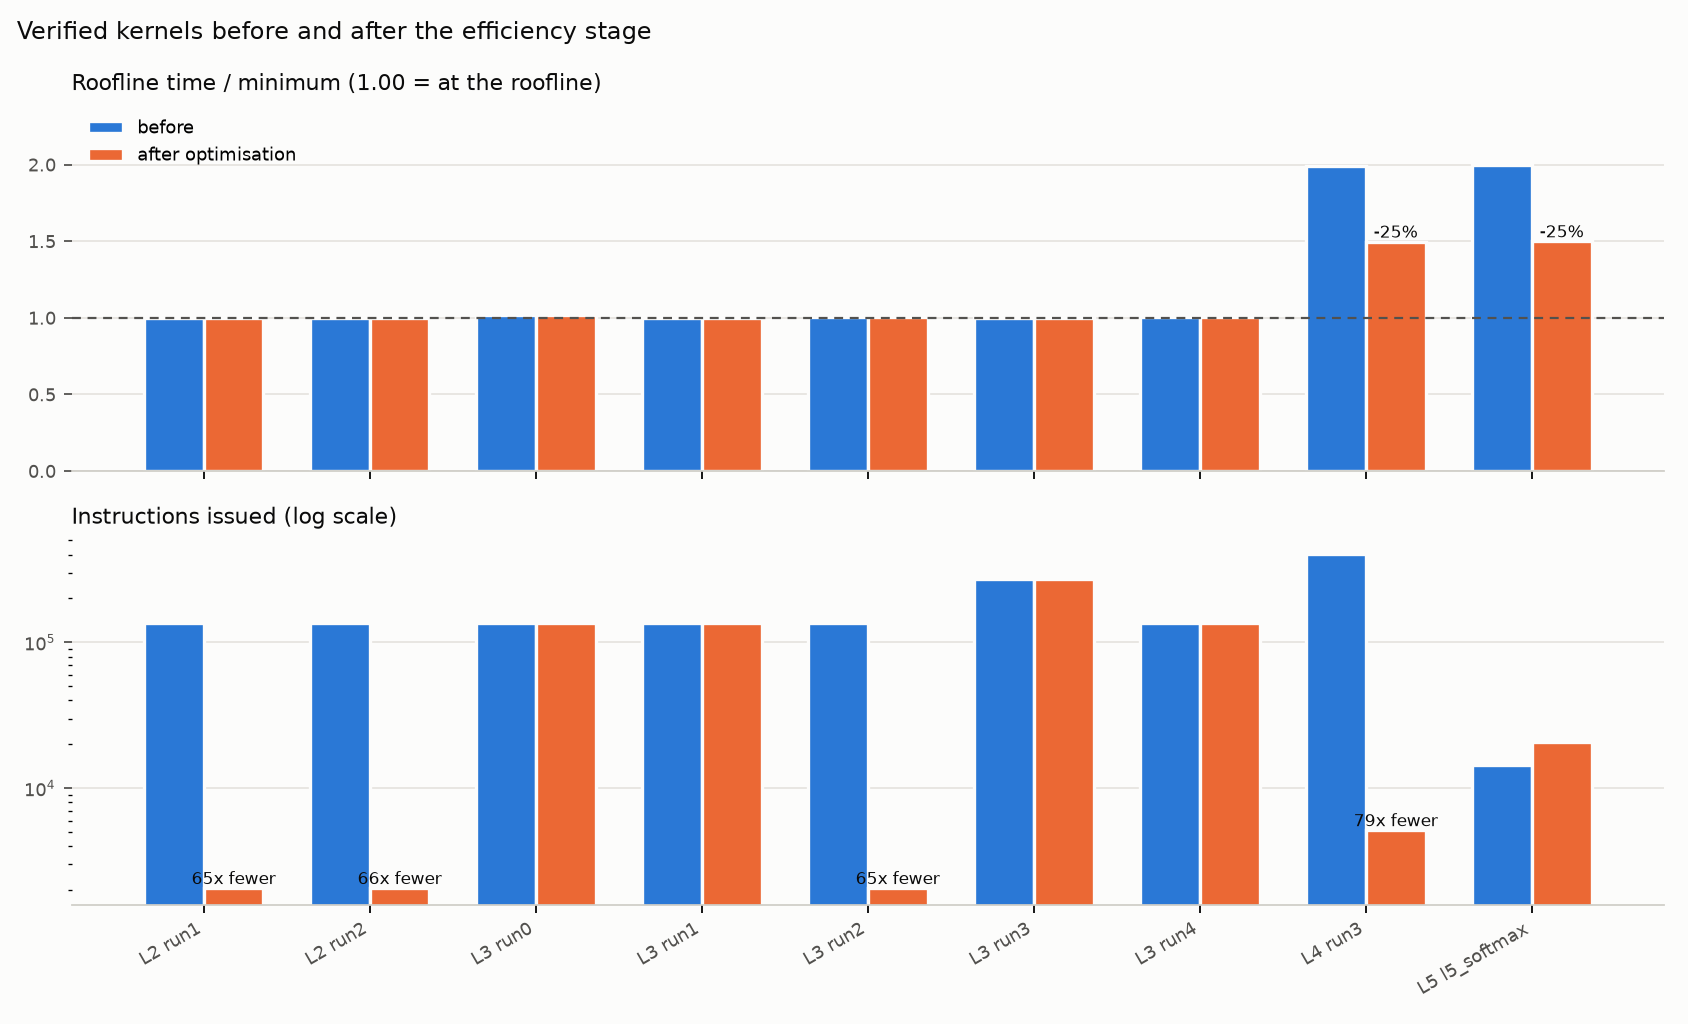
\includegraphics[width=0.92\linewidth]{fig-opt2.png}
\caption{Optimiser v2. Top: roofline time; bottom: instructions (log scale).}
\label{fig:opt}
\end{figure}

\subsection{Token use}
On a real run (ours, run 4, L1--4; Figure~\ref{fig:tok}) the largest prompt is 706 tokens, 13\% of the
input budget; over all five v2 runs on L1--4 the largest is 779 tokens, under 15\%. Spend per section:
task $\approx$70--130, code 130--360, feedback 80--240, ledger 40--70 (only on repeats). \textbf{In Stage~A
the budget never binds}: the model knows NumPy, so no documentation is needed. The context-selection
problem is real in Stage~B, where the model invents NKI APIs (\S\ref{sec:stageb}). We state this rather
than claim to have solved it here.

\begin{figure}[h]
\centering
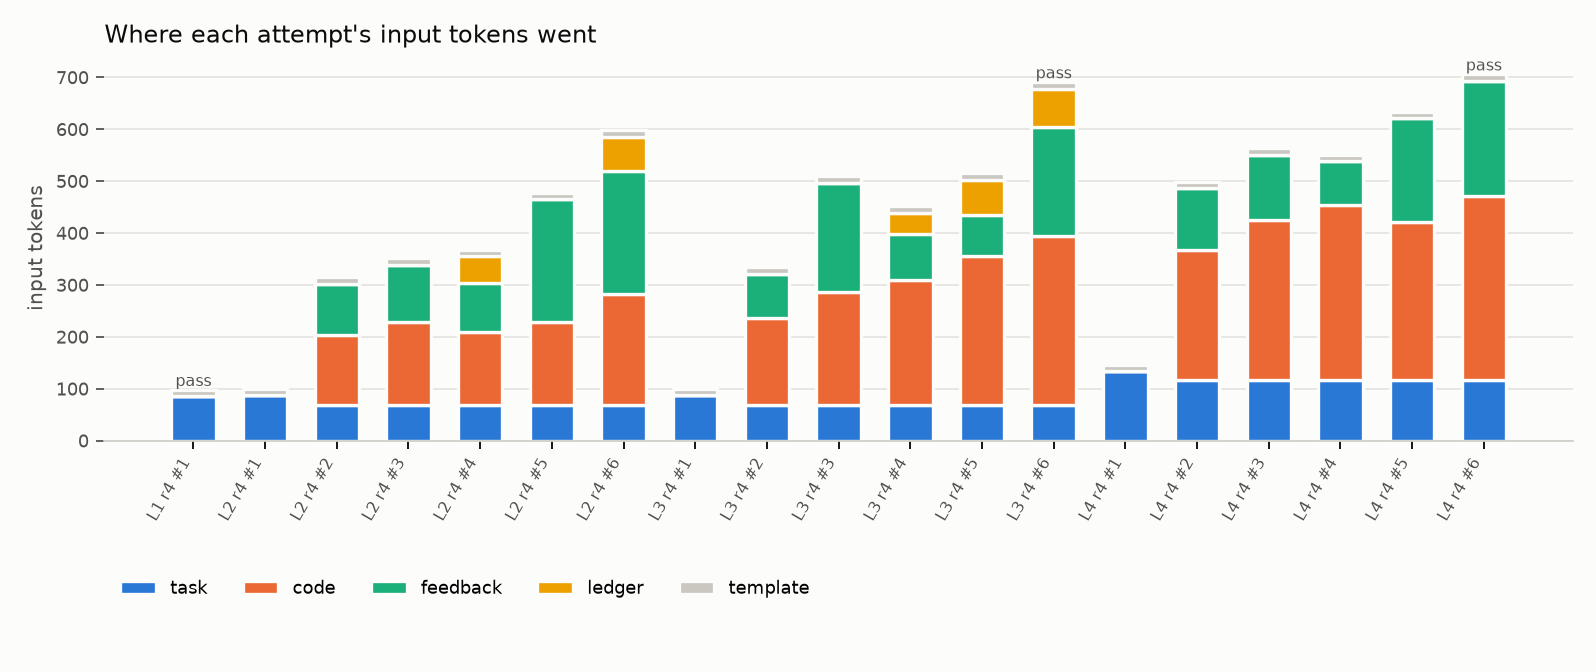
\includegraphics[width=0.92\linewidth]{fig-tokens-run4.png}
\caption{Input tokens per attempt by section, real run (ours, run 4, L1--4).}
\label{fig:tok}
\end{figure}

\subsection{Calibration}
Every v2 \code{verified} kernel was right. The \code{dev-only} kernels were not wrong but slow: all
three ours L7 dev-only kernels (seat-130 runs 1 and 3, seat-133 run 4) failed holdout only by the 20\,s
per-case timeout of a per-element triple loop, and re-check as slow-but-correct (10/10 holdout with a
long timeout, \E{21}, \E{24}). The 0.3 confidence was too low; v3's 120\,s holdout timeout removes the
artefact. Section~\ref{sec:kb} adds an external check of the same verdicts.

%==============================================================================
\section{Analysis}
\label{sec:analysis}

\subsection{Failure taxonomy}
Table~\ref{tab:tax} counts failed attempts per mode over all v2 runs (\code{TAXONOMY.md}).

\begin{table}[h]
\centering
\resizebox{\linewidth}{!}{% generated by scripts/taxonomy.py
\begin{tabular}{@{}lrrrrrrrrrrr@{}}
\toprule
Failure mode & naive L1 & naive L2 & naive L3 & naive L4 & ours L1 & ours L2 & ours L3 & ours L4 & ours L5 & ours L6 & ours L7 \\
\midrule
banned reduction & -- & 23 & 11 & 13 & -- & 9 & 9 & 7 & 10 & -- & -- \\
hid the tiling & 8 & -- & 1 & 10 & 3 & -- & -- & 5 & 12 & 7 & 14 \\
crash & -- & -- & 1 & 6 & -- & 5 & 1 & 12 & 10 & 12 & 4 \\
partial tile / bounds & -- & -- & -- & -- & -- & -- & 1 & -- & -- & -- & 1 \\
accumulator across tiles & -- & -- & 5 & -- & -- & 3 & 7 & 3 & 3 & -- & -- \\
floating point & -- & -- & -- & -- & -- & -- & 3 & 6 & -- & -- & -- \\
\bottomrule
\end{tabular}
}
\caption{Failed attempts by mode (\code{scripts/taxonomy.py}).}
\label{tab:tax}
\end{table}

\noindent Readings. (1) The first wall at every level is a banned reduction (\code{np.sum}/\code{np.max}).
(2) naive stops on rule violations: a verdict alone does not get the model past a rule. ours stops on
deeper problems: crashes at partial tiles (L5--L7) and floating point and accumulator errors (L4).
(3) No attempt is ``unexplained wrong numbers''; the diagnoses of \E{9} and \E{12} cover what the model
actually does. (4) A repair fixed the error shown but lowered the number of passing cases in 32 of 128
ours repairs and 9 of 62 naive repairs: our directives produce bigger moves, which also break more.

\subsection{Why L1--L3 work and L4 is a wall}
L1--L3 need one pass and one idea each; the banned reduction is the only wall, and the directive gives
the column loop. RMSNorm needs four hurdles cleared in order (\E{25}): (1) no \code{np.mean} of the
squares; (2) normalise a tile without broadcasting; (3) a statistic over the whole row, not one tile;
(4) float64 squares for $\pm10^{18}$. Hurdle 2 is the largest, 13 of 37 v2 failures. The natural code
divides a (rows, cols) tile by a (rows,) vector; that crashes, \code{.reshape(-1,1)} or
\code{np.newaxis} fixes the crash but breaks the layout rule, reverting crashes again; runs 2 and 3 never
left this loop. Under the rules a per-row vector can only be applied one column at a time, and nothing
told the model so. Two passes, a rule that bans the natural form, a numeric trap and fixes that interact:
each hurdle is clearable, but all four within eight attempts happened once in five runs.

\subsection{Oscillation}
v3's ``rewrite the loop structure'' lets the model make the structural change v2 forbade, and the
model then reached correct numbers on L4 for the first time; but a rewrite also drops fixes made
earlier, so cleared failure classes return. The ledger records what failed, not what must stay fixed.
A ``must keep'' list would address this; we did not add it (\S\ref{sec:limits}).

\subsection{\texorpdfstring{Determinism, and why best-of-$n$ is a no-op}{Determinism, and why best-of-n is a no-op}}
Six replies to one prompt were byte-identical (\E{27}); runs 1 and 2 were identical attempt by attempt
until the first divergence (\E{10}). Requesting $N$ samples per prompt therefore buys $N$ copies at
$N\times$ the cost, contrary to the upstream README's ``Qwen3's samples differ''. Diversity must come
from the prompt, which is why each run uses its own wording (run 3 and 4 solve L1 in one attempt because
their wordings never trigger \code{np.asarray}). A prompt-varied best-of-$n$ remains open; at about
25 tokens/s per server it trades depth (12 sequential repairs) for breadth.

\subsection{Stage B (NKI), by teammates}
\label{sec:stageb}
The upstream NKI agent scores $r = 0.1[\text{parses}] + 0.2[\text{rules}] + 0.2[\text{runs}] +
0.5\cdot\text{shapes passed}/\text{shapes}$, where ``runs'' becomes true once any shape simulates. So the
recurring 0.30 means \emph{every shape crashed}, not ``ran but wrong'' as its README says. The crashes
fall into four kinds: invented functions (\code{nisa.multiply}), invented arguments
(\code{transpose\_moving=}), real calls with violated constraints (\code{nc\_matmul} output outside
PSUM, \code{dma\_copy} element mismatch), and the partial-tile trap. On NKI the failures are API misuse,
and here the 8k page does bind. Unchanged upstream on seat-130: L1 0/5 (0.30), L2 4/5, L3 0/5 (0.30),
L4 0/5 (0.62) (\E{20}). A teammate's feedback changes solved NKI L4 (1/5 with v2, \E{17}, \E{24}) and
took NKI L1 from 0/5 to 5/5 with v5, whose feedback names the wrong \code{.ap()} strides. The key L4
change mirrors ours: the stock repair prompt said ``change exactly what the checker names and keep
everything else identical'' while the checker asked for a new loop structure, and the model obeyed the
first in 72 of 80 L4 attempts. Our own v2 repair prompt ended with the same sentence, which motivated
v3 change~1.

%==============================================================================
\section{Judged by the organizers' checker}
\label{sec:kb}

(\E{29}.) We ran every verified kernel from every run, and the dev-only L7 kernels, through the
organizers' \code{kernelbench.py}: their signatures, references and cases, a per-element relative
tolerance of $10^{-4}$, and their rule scan.

\begin{table}[h]
\centering\small
\begin{tabularx}{\linewidth}{@{}l>{\raggedright\arraybackslash}p{5.2cm}Y@{}}
\toprule
Level & Result & Cause \\
\midrule
L1, L2, L3 & every verified kernel 32/32 & -- \\
L6 & the naive verified kernel passes & -- \\
L4 & 0/32 (every call raised) & signature: organizers \code{kernel(x, eps=1e-6)}, ours \code{kernel(x, g, eps)} \\
L8 & (same mismatch) & organizers \code{kernel(x, eps=1e-5)}, ours \code{kernel(x, g, b, eps)} \\
L7 & all seven dev-only kernels 4/10; even our hand matmul 5/10 & float32 products; relative errors $5$--$8\times10^{-4}$ on outputs that happen to be near zero \\
L10 & the four naive verified kernels 3/4 & relative error $1.05\times10^{-4}$ \\
\bottomrule
\end{tabularx}
\caption{Our kernels under \code{kernelbench.py}.}
\label{tab:kb}
\end{table}

So under the organizers' checker we reliably clear L1, L2, L3 and L6; L4 and L8 need the signature
aligned; L7 and L10 need float64 products and sums. The disagreement on L7/L10 is a difference of criterion,
not a bug in either checker: our proven bound $\gamma_k s$ scales with the magnitudes that enter the
computation, so on outputs near zero it admits an absolute error that a per-element relative tolerance
of $10^{-4}$ rejects. Ours is the principled bound for a float32 algorithm; theirs is the rule that is
scored. A teammate's differential script (\code{scripts/differential.py}, every kernel in
\code{kernels/hand}, \code{kernels/broken} and \code{kernels/redteam} through both checkers) finds 36 of 41 kernels with the same
verdict.

\paragraph{Response: v4, the final agent} (branch \code{v4}, \code{174153fd32}) is v3 plus alignment with the
organizers' checker. L4 and L8 use their signatures, \code{kernel(x, eps=1e-6)} and
\code{kernel(x, eps=1e-5)}, and their references. A kernel is reported verified only if
\code{kernelbench.py} (loaded from the seat pod) also passes it, and its failures become one directive
(``callable as \code{kernel(x, eps=1e-6)}'', ``compute in float64'', \dots); the hand matmul multiplies in
float64. A first attempt to emulate their tolerance inside our harness failed 10 self-tests, because
their references differ per level (L1 is computed in float32); the only faithful emulation is their
checker itself, so the gate calls it. v4 runs (L4 and L7 on seat-130; L8--L10 on teammates' pods) are in
progress; results are \textbf{pending}.

%==============================================================================
\section{Limitations and next steps}
\label{sec:limits}
\begin{itemize}
  \item \textbf{v3's six changes are confounded, and its win is small.} They were introduced together, so
        the E26 verdict (3/9 vs 1/25) can only say that v3 as a whole is better; most of the gain is L6. One change per arm did not fit in the remaining time
        and compute.
  \item \textbf{The Stage~A budget never binds} (706 tokens at most). Our token discipline is measured,
        not stressed; Stage~B is where it would matter.
  \item \textbf{One small model, one server, five runs per cell}, and the runs are near-deterministic
        (\E{10}), so rates carry less information than their denominators suggest.
  \item \textbf{Not run:} a ``must keep'' list against oscillation, and prompt-varied best-of-$n$.
  \item \textbf{Deliberately not added:} a memory of past mistakes in the first prompt. It puts rules
        back into the prompt, the thing that makes the model audit itself into silence, and it would need
        its own arm.
  \item \textbf{Criterion mismatch} with the organizers' checker on L4/L7/L8/L10 (\S\ref{sec:kb}); v4 closes it
        by gating on their checker, but its runs are pending.
\end{itemize}

%==============================================================================
\section{Reproducibility}
Repository: \url{https://github.com/LiYou22/kernel-agent}. Locally, without a model (about 2 minutes):

\begin{small}
\begin{verbatim}
uv sync
uv run pytest -q                                            # 59 passed (main)
uv run python -m kagent.harness 4 kernels/hand/l4_rmsnorm.py
uv run python -m kagent.harness 3 kernels/broken/l3_overwrite_per_tile.py --fixes
uv run python -m kagent.agent --levels 1 2 --scripted tests/scripts/demo.json \
    --out runs/demo.jsonl
uv run python scripts/plot_tokens.py runs/demo.jsonl
uv run python scripts/list_cases.py                         # regenerates EVALSET.md
\end{verbatim}
\end{small}

\noindent On a seat pod (Qwen3-8B on vLLM via \code{/workspace/serve.sh}):

\begin{small}
\begin{verbatim}
scripts/sync.sh                    # push tracked files to /workspace/stageA
scripts/launch.sh ours 1 2 3 4     # 5 runs per level
scripts/launch.sh naive 1 2 3 4    # ablation: verdict sent back verbatim
scripts/fetch.sh                   # logs to results/$POD/
R=results/seat-130
uv run python scripts/analyze.py ours=$R/ours-L1234-seat-130.jsonl \
    naive=$R/naive-L1234-seat-130.jsonl --recheck
uv run python scripts/taxonomy.py ours=... naive=... --md TAXONOMY.md
\end{verbatim}
\end{small}

\noindent Code versions (hash of \code{kagent/*.py}, logged with every result): v2 \code{e22ccab872}
(\code{main}; all comparisons in Tables~\ref{tab:main}, \ref{tab:l510}); v3 \code{29fd8d90d5} (branch
\code{v3}; earlier \code{ea9befddac}, \code{eddb241adf}; Table~\ref{tab:v3res}); v4 \code{174153fd32} (branch
\code{v4}, the final agent; runs pending). Pod: Python 3.13, NumPy 2.4.6. Never send
\code{seed} to the server.

%==============================================================================
\clearpage
\appendix
\section{Experiment log index}
One line per entry; full entries in \code{notes/notes.tex}.

{\small
\noindent\begin{tabularx}{\linewidth}{@{}l>{\raggedright\arraybackslash}p{5.0cm}Y@{}}
\toprule
\# & Title & Finding \\
\midrule
E1 & Hand kernels pass & L1--L3 40/40, 28/28, 24/24; worst error $8.4\times10^{-8}s$ \\
E2 & float32 accumulation vs tolerance & constant $10^{-5}$ rejected a correct float32 row sum (superseded by E7) \\
E3 & Deliberate bugs are caught & 9 bugs, each with the expected kind and key phrase; 14 tests \\
E4 & Misleading first diagnostics & wrong tag blame, wrong tile claim; a wrong explanation misleads the fix \\
E5 & \code{seed} kills the server & Neuron vLLM engine dies; never send \code{seed} \\
E6 & First model call, L1 & 107 tokens; 40/40 correct but \code{np.asarray}: one repair needed \\
E7 & Proven error bounds & $\gamma_k s$ replaces the constant; hand kernels $\le47\%$ of the bound \\
E8 & Efficiency accounting & hand kernels at the FLOP and traffic minimum \\
E9 & Per-tile overwrite & first live bug the translator could not name; new verified hypothesis \\
E10 & Runs are not independent & byte-identical code across runs; vary the wording per run \\
E11 & One harness version & version hash on every result; AppleDouble files fixed \\
E12 & Two compounding bugs & verified hypotheses win at $\ge50\%$ coverage \\
E13 & Directive induces a violation & ``or divide by the max'' led to \code{np.max}; one safe remedy \\
E14 & Efficiency stage, roofline & $t=\max(\text{bytes},\text{FLOPs}/222)$; online softmax is a win \\
E15 & Per-element loops looked free & 5 of 6 verified L2/L3 kernels per-element, $\sim65\times$ instructions \\
E16 & Optimiser v1 & 0 of 13 rewrites accepted \\
E17 & PR~\#1 solves NKI L4 & ``change only that'' blocked loop rewrites (72/80) \\
E18 & v2 ours L1--4 final & 5/5, 4/5, 5/5, 1/5; largest prompt 779 tokens \\
E19 & Optimiser v2 & 5 of 11 accepted; up to $79\times$ fewer instructions \\
E20 & Upstream NKI agent on seat-130 & L1 0/5, L2 4/5, L3 0/5, L4 0/5 (0.62) \\
E21 & First naive and L5--7 results & naive repeats verbatim violations; L7 dev-only was slow, not wrong \\
E22 & Deliverables & 207 + 156 cases; max prompt 706 tokens (13\%); taxonomy \\
E23 & v3 built & five changes from live evidence; 61 tests \\
E24 & Final v2 results & ours 15/20 vs naive 4/20; L5--7 0/5 on two seats; red-team alias fix \\
E25 & Why L4 is a wall & four hurdles; broadcast is the largest; v3 oscillates \\
E26 & Pre-registered v3 rule & better iff $\ge2/9$ on L4--L6 \\
E27 & Best-of-$n$ is a no-op & 6 identical replies to one prompt \\
E28 & v3 run 1 & 0/3, but L4 24/24 numbers; one rule left \\
E29 & Organizers' checker & L1--L3, L6 pass; L4/L8 signature; L7/L10 need float64; v4 gates on it \\
E30 & v3 verdict (E26 rule) & 3/9 vs v2's 1/25 on L4--L6: v3 adopted; v4 = v3 + organizers' gate \\
\bottomrule
\end{tabularx}}

\end{document}
